\documentclass{statsoc}

\usepackage[a4paper]{geometry}
\usepackage{graphicx}
\usepackage[textwidth=8em,textsize=small]{todonotes}
\usepackage{amsmath}
\usepackage{dsfont}
\usepackage{natbib}
\usepackage{amsbsy}
\usepackage{graphicx,amsmath,amssymb,fullpage, amsfonts,bbm,bbold}
\usepackage{lineno}
\usepackage{color}
\usepackage{enumerate}
\usepackage{tikz}
\usetikzlibrary{arrows}
\usetikzlibrary{positioning}
\usepackage{dsfont}
\usepackage{longtable}
\usepackage{bm}
\usepackage{mwe}
\usepackage{float}
\usepackage[hyperindex,breaklinks]{hyperref}
\usepackage{pdflscape}
\newdimen\nodeDist
\nodeDist=25mm
\usepackage{bm}
\usepackage{natbib}
\usepackage{algorithm}
\usepackage{algpseudocode}
\def\argmin{\operatornamewithlimits{arg\,min}}
\DeclareMathOperator{\iid}{\stackrel{\mbox{\tiny iid} }{\sim}}
\newcommand{\logit}{\mbox{logit}}
\newcommand{\B}{\mathbf{B}}
\newcommand{\bPsi}{\mathbf{\Psi}}
\newcommand{\bbeta}{\boldsymbol{\beta}}
\newcommand{\X}{\mathbf{X}}
\newcommand{\Y}{\tilde{Y}}
\newcommand{\tepsilon}{\tilde{\epsilon}}
\newcommand{\blambda}{\mathbf{\lambda}}
\newcommand{\Z}{\mathbf{Z}}
\newcommand{\br}{\mathbf{r}}
\newcommand{\bv}{\mathbf{b}}
\newcommand{\f}{\mathbf{f}}
\newcommand{\btheta}{\boldsymbol{\theta}}
\newcommand{\epsy}{\epsilon}
\newcommand{\epsz}{\nu}
\newcommand{\z}{\mathrm{z}}
\newcommand{\cc}{\mathbb{c}}
\newcommand{\y}{\mathrm{y}}
\newcommand{\bSigma}{\boldsymbol{\Sigma}}
\newcommand{\probit}{\mbox{probit}}
\newcommand{\hiw}{\mbox{{\small\textsc{HIW}}}}
\newcommand{\iw}{\mbox{{\small\textsc{IW}}}}
\newcommand{\N}{\mbox{{\small\textsc{N}}}}
\newcommand{\T}{\mbox{{\small\textsc{T}}}}
\newcommand{\C}{\mbox{{\small\textsc{C}}}}
\newcommand{\Ga}{\mbox{{\small\textsc{Ga}}}}
\newcommand{\IG}{\mbox{{\small\textsc{IG}}}}
\newcommand{\Be}{\mbox{{\small\textsc{Be}}}}
\newcommand{\Ber}{\mbox{{\small\textsc{Ber}}}}
\newcommand{\dd}{\bm{d}}
\newcommand{\E}{\mbox{E}}
\newcommand{\V}{\mathbf{V}}
\newcommand{\Polya}{P\'olya}
\newcommand{\p}{\bm{p}}
\newcommand{\w}{\bm{w}}
\newcommand{\eeta}{\bm{\eta}}
\newcommand{\n}{\bm{n}}
\newcommand{\alphavec}{\bm{\alpha}}
\newcommand{\red}[1]{{\color{red} #1}}
\newcommand{\nn}{\bm{n}}

\newcommand{\etavec}{\bm{\eta}}
\newcommand{\wvec}{\bm{\omega}}
\newcommand{\I}{\mathbf{I}}
\newcommand{\Tau}{\mathrm{T}}
\newcommand{\quantile}{\text{Quantile}}
\newcommand{\defeq}{\mathrel{\mathop:}=}
\newcommand{\norm}[1]{\left\lVert#1\right\rVert}
\newcommand{\dequal}{\,{\buildrel D \over =}\,}
\newcommand{\x}{\mathrm{x}}
\newcommand{\sayan}[1] {{\textcolor{red}{ #1}}}
\newtheorem{theorem}{Theorem}
\newtheorem{claim}{Claim}
\newtheorem{proposition}{Proposition}
\newtheorem{lemma}{Lemma}
\newtheorem{corollary}{Corollary}
\newtheorem{definition}{Definition}
\newtheorem{assumption}{Assumption}
\newtheorem{remark}{Remark}
\newenvironment{example}[1][Example]{\begin{trivlist}
\item[\hskip \labelsep {\bfseries #1}]}{\end{trivlist}}
%\newenvironment{remark}[1][Remark]{\begin{trivlist}
%\item[\hskip \labelsep {\bfseries #1}]}{\end{trivlist}}
%\newcommand\independent{\protect\mathpalette{\protect\independenT}{\perp}}
%\def\independenT#1#2{\mathrel{\rlap{$#1#2$}\mkern2mu{#1#2}}}

\usetikzlibrary{calc}

\definecolor{block}{RGB}{0,162,232}

\newenvironment{blockmatrix}{%
  \left[%
  \vcenter\bgroup\hbox\bgroup
  \tikzpicture[
    x=1.5\baselineskip,
    y=1.5\baselineskip,
  ]%
}{%
  \endtikzpicture
  \egroup
  \egroup
  \right]%
}

% \block[#1](#2,#3)#4(#5,#6)
% #1:      fill color
% (#2,#3): lower left corner
% #4:      text in the middle
% (#5,#6): size of the block
\newcommand*{\block}[1][block]{%
  \blockaux{#1}%
}
\def\blockaux#1(#2,#3)#4(#5,#6){%
  \draw[fill={#1}, draw=white]
  let \p1=(#2,#3),
      \p2=(#5,#6),
      \p3=(#2+#5,#3+#6),
      \p4=(#2+#5/2,#3+#6/2)
  in
    (\p1) rectangle (\p3)
    (\p4) node {$#4$}
  ;%
}


\title[P\'olya Inverse Gamma]{Bayesian Inference for P\'olya Inverse Gamma Models}
\author[Jianeng Xu {\it et al.}]{Jianeng Xu}
\address{University of Chicago,
USA.}



\begin{document}
\begin{abstract}
Probability density functions that include the gamma function are widely used in statistics and machine learning. The normalizing constants of gamma, inverse gamma, beta, and Dirichlet distributions all include model parameters as arguments in the gamma function; however, the gamma function does not naturally admit a conjugate prior distribution in a Bayesian analysis, and statistical inference of these parameters is a significant challenge.  In this paper, we construct the P\'olya-inverse Gamma (P-IG) distribution as an infinite convolution of Generalized inverse Gaussian (GIG) distributions, and we represent the reciprocal gamma function as a scale mixture of normal distributions.  As a result, the P-IG distribution yields an efficient data augmentation strategy for fully Bayesian inference on model parameters in gamma, inverse gamma, beta, and Dirichlet distributions.  To illustrate the applied utility of our data augmentation strategy, we infer the proportion of overdose deaths in the United States attributed to different opioid and prescription drugs with a Dirichlet allocation model.\\

\textit{Keywords:} P\'olya inverse Gamma, Latent Dirichlet Allocation,  Gamma shape, Generalized Gamma Convolutions.
\end{abstract}


\section{Introduction}
\label{sec:Introduction}
Gamma, inverse gamma, beta, and Dirichlet probability distributions are core components of many Bayesian statistical and machine learning models.  The normalizing constants of these distributions depend on gamma functions whose arguments include shape (gamma, inverse gamma) and concentration (beta, Dirichlet) parameters.  Bayesian learning of parameters nested inside the gamma function presents significant technical difficulties, since there is no known conjugate prior distribution.  In fact, inferring the shape parameter in the gamma distribution is a long-studied problem in Bayesian inference \citep{damsleth1975conjugate, rossell2009gaga, miller2018fast}.  

In this paper, we develop the theoretical and algorithmic foundation of a \Polya-inverse Gamma (P-IG) data augmentation scheme for fully Bayesian inference of shape and concentration parameters in gamma, inverse gamma, and Dirichlet models, respectively.  P-IG data augmentation may be utilized to design efficient Markov chain Monte Carlo (MCMC) algorithms in latent Dirichlet allocation \citep{blei2003latent}, Beta-negative binomial models \citep{zhou2012beta}, and Gamma-Gamma (GaGa) hierarchical models \citep{rossell2009gaga}.  It adds to the literature on Bayesian computation with auxiliary variables, which have proven useful in computing posterior distributions in logistic regression \citep{polson2013bayesian}, multinomial factor models \citep{holmes2006}, support vector machines \citep{mallick2005bayesian, polson2011data}, and dependent multinomial models \citep{linderman2015dependent}.   

The P-IG distribution is defined as an infinite convolution of Generalized inverse Gaussian (GIG) distributions and has direct application to gamma shape inference.  Our data-augmentation scheme builds on distributional results of \cite{hartman1976completely}  and \cite{roynette2005couples}, who provide a representation of the reciprocal gamma function as a scale mixture of normals. This adds to scale mixtures results in Bayesian inference, see \cite{andrews1974scale}, \cite{barndorff1982normal}, \cite{west1987scale}, and \cite{polson2013bayesian}. Scale mixtures of normals are increasingly used in modeling complex high-dimensional distributions, and \cite{bhattacharya2016fast} provide fast sampling strategies, adding to the practical use of scale mixture distributions in scalable stochastic simulations.  Equivalently constructed scalable PG sampling schemes are provided in \cite{windle2014sampling} and \cite{glynn2018bayesian}. 

To illustrate the applied utility of our data augmentation strategy, we use a multinomial - Dirichlet  model to estimate the proportion of overdose deaths in the United States attributed to different opioid and prescription drugs.  Robust quantification of uncertainty in the number of deaths attributed to opioids is of great interest to the public health community, and our P-IG approach provides a full posterior distribution, avoiding approximate EM-style algorithms such as \cite{minka2000estimating} or the simulation approach of \cite{miller2018fast} and that taken by \cite{rossell2009gaga} in the class of GaGa models.  We also present an application of gamma shape inference \citep{west1992hyperparameter, miller2018fast}. 

The rest of our paper is outlined as follows: Section \ref{sec:P-IG} defines the class of P-IG distributions; Section \ref{sec:Conentration_Inference} constructs data augmentation strategies in hierarchical multinomial-Dirichlet models, developing a parameter expanded Gibbs sampler for fully Bayesian inference of Dirichlet concentration parameters; Section \ref{sec:Shape_Inference} presents an augmentation strategy for fully Bayesian inference of the shape parameter in the gamma distribution; Section \ref{sec:Application} presents an analysis of the opioid and prescription drug overdose data; and Section \ref{sec:Discussion} concludes with directions for future research. 

\section{The P\'olya-Inverse Gamma (P-IG) Distribution Class}
\label{sec:P-IG}
In this section, we present the theoretical development of the P-IG distribution class, defining the P-IG distribution by the form of its integral transform.  In Section \ref{subsec:PIG_d0}, we define a specific case of the P-IG distribution and prove that it is an infinite convolution of independent GIG distributions; in Section \ref{subsec:PIG_dc}, the general class of \Polya-Inverse Gamma distributions is constructed with an exponential tilting of the special case defined in Section \ref{subsec:PIG_d0}.         

\subsection{The P-IG(0) distribution}
\label{subsec:PIG_d0}
Let P-IG(0) denote the \Polya-inverse Gamma distribution. The parameter, which is a tilting parameter fixed at zero in this case, will be discussed in greater detail in Section \ref{subsec:PIG_dc}.  
\begin{definition}
Random variable $\omega$ has a  P\'olya-inverse Gamma distribution, P-IG(0), if and only if its density $f(\omega)$ satisfies the following identity
\begin{equation}\label{LT_b_0}
\int_{0}^\infty e^{-\omega t^2} f(\omega) d \omega = \prod_{k=1}^\infty \left(1 + \frac{t}{k}\right) e^{- \frac{t}{k}}.
\end{equation}
for any $t \geq 0$.
\end{definition}

\begin{remark}
\label{rmk:remark_1}
One of the product representations for the reciprocal Gamma function is,
$$
\frac{1}{\Gamma(z)} = z e^{\gamma z}\prod_{k=1}^\infty \left(1 + \frac{z}{k}\right) e^{-\frac{z}{k}}, \, z\in \mathbb{C}\slash \{0\}
$$
where $\gamma = -\psi(1) \approx 0.57721$ is the Euler-Mascheroni constant and $\psi(\cdot)$ is the digamma function. Therefore, the reciprocal Gamma function can be viewed as a expectation function with respect to the P-IG(0), 
$$
\frac{1}{\Gamma(t)} = \int_{0}^\infty te^{-\omega t^2 + \gamma t} f(\omega) d \omega = E\left(te^{-W t^2 + \gamma t}  \right)
$$
for $t>0$ and $W\sim \text{P-IG(0)}$.
\end{remark}

\begin{lemma}\label{lemma1}
A P-IG(0) random variable can be represented as an infinite sum of inverse gamma (IG) distributions. Since the inverse gamma distribution is a special case of the generalized inverse Gaussian (GIG)\footnote{The inverse gamma (IG) is a special case of the three-parameter generalized inverse Gaussian distribution, GIG$\left(p, a, b\right)$, with density function
$$
f\left(x\right) \propto x^{p - 1}\exp\left\{-\frac{1}{2}\left(a x + bx^{-1}\right)\right\}, \quad a,b,x > 0, p\in\mathbb{R}.
$$
} distribution, it follows that 
\begin{equation}
W \overset{d}{=}\sum_{k=1}^\infty IG\left(\frac{3}{2}, \frac{1}{4k^2}\right)
\overset{d}{=}   \sum_{k=1}^\infty GIG
\left(-\frac{3}{2}, 0,  \frac{1}{2k^2}\right).
\end{equation}
\end{lemma}
\begin{proof}
See Appendix \ref{lemma_proof}.
\end{proof}


\subsection{The General P-IG(c) Class}
\label{subsec:PIG_dc}
We construct the general class of P-IG distributions, P-IG$\left(c\right)$, by exponentially tilting the P-IG$(0)$ class.  The exponential tilting strategy -- similar to the one used by \citet{polson2013bayesian} -- allows a second parameter $c \in \mathbb{R}$ to inform a priori the precision of the P-IG random variable.        
\begin{definition}
\label{def:PG_dc}
The P-IG$(c)$ distribution is constructed as an exponential tilting of the P-IG(0) density. Its density function is
\begin{equation}
f\left(\omega \mid c\right) \propto \exp\left(- c^2 \omega\right) f(\omega),\, \omega,c >0.
\end{equation}
The normalizing constant, namely $1/E\left[\exp\left(-c^2 W_0\right)\right]$ where $W_0$ is a P-IG(0) random variable, can be calculated using the integral identity in (\ref{LT_b_0}). Similarly, the integral identify of P-IG$(c)$ is given by
\begin{equation}
E(e^{-t^2 W_c}) = \prod_{k=1}^\infty \left( \frac{k + \sqrt{t^2 + c^2}}{k + c} \right) e^{-\frac{\sqrt{t^2 + c^2}-c}{k}}.
\end{equation}
\end{definition}

Our main result, presented in Theorem \ref{thm:theorem_1}, is that a random variable $X\sim$ P-IG$(c)$ may be constructed from an infinite sum of independent GIG-distributed random variables.  The power of the result lies in the ability to identify previously unknown conditional posterior distributions in Bayesian inference. 

\begin{theorem}
\label{thm:theorem_1}
The P-IG$(c)$ class of distributions can be constructed as an infinite sum of generalized inverse Gaussian (GIG) distributions as follows
$$
\mbox{P-IG}(c) \overset{d}{=} \sum_{k=1}^\infty GIG\left(-\frac{3}{2}, 2c^2, \frac{1}{2k^2}\right).
$$
\end{theorem}
\begin{proof}
See Appendix \ref{proof_thm1}.
\end{proof}


\begin{remark}
If $W\sim$ P-IG$(c) \overset{d}{=} \sum_{k=1}^\infty GIG\left(-\frac{3}{2}, 2c^2, \frac{1}{2k^2}\right)$, then its expectation is given by
\begin{align*}
E(W) &= \sum_{k=1}^\infty \frac{1}{2ck}\frac{K_{-\frac{1}{2}}(c/k)}{K_{-\frac{3}{2}}(c/k)}\\
&= \sum_{k=1}^\infty \frac{1}{2ck} \frac{c/k}{1 + c/k} \\
&= \frac{\gamma + \psi(c + 1)}{2c},
\end{align*}
where $K_v(\cdot)$ is the modified Bessel function of the second kind. $\psi(\cdot)$ is digamma function.
\end{remark}

\begin{remark}
\cite{roynette2005couples} prove the existence of an infinitely divisible distribution function $H(\omega) = H(\omega, a)$, such that 
$$
\frac{\Gamma(a)}{\Gamma(a+t)} e^{\psi(a)t} = \int_0^\infty e^{-t^2 \omega} H(d\omega, a).
$$
This is related to a more general product representation for the reciprocal gamma function, 
\begin{equation}
\frac{\Gamma(a)}{\Gamma\left(a + t\right)} = e^{-\psi(a)t}\prod_{k=0}^{\infty}\left( 1 + \frac{t}{a+ k} \right)e^{-\frac{t}{a+k}}.
\end{equation}
Note that the representation in Remark \ref{rmk:remark_1} is a special case with $a = 1$.
\end{remark}

\section{Inferring concentration parameters in multinomial-Dirichlet models}
\label{sec:Conentration_Inference}
In this section, we develop Markov chain Monte Carlo (MCMC) algorithms for fully Bayesian inference of the concentration parameter vector in the Dirichlet distribution.  Such inference problems commonly arise in applied analyses of categorical data.  Section \ref{subsec:Model_Framework} presents the general hierarchical multinomial-Dirichlet model class for which the P-IG data augmentation scheme may be utilized.  Section \ref{subsec:Data_Augmentation} develops a parameter expanded Gibbs sampler for inferring the concentration parameter in the Dirichlet distribution.  

\subsection{A hierarchical multinomial-Dirichlet model class}
\label{subsec:Model_Framework}
The multinomial-Dirichlet framework presented herein is closely related to the latent Dirichlet allocation model of \citet{blei2003latent} for topic modeling in text data, and we use text analysis as a motivating context.  Suppose that for document $m \in \{1, \ldots, M\}$, each of $N_m$ words in the document is independently allocated to $K$ topics conditional on probability vector $\p_m = \left(p_{m1}, p_{m2}, \ldots, p_{mK}\right)$.  For each document $m$, the number of words allocated to each topic, $\nn_m = \left(n_{m1}, \cdots, n_{mK}\right)$, is modeled with a multinomial distribution.  The sampling model for the count vector $\nn_m$ is then a multinomial distribution given probability vector $\p_m$,  
\begin{align}
    \nn_m \mid \p_m  \sim \text{Multinomial}\left(\p_m\right).
\end{align}
The probability vector $\p_m$ is the proportional allocation of each document to the $K$ topics.  In a Bayesian analysis, the probability vector for each document $\p_m$ is typically assigned a Dirichlet distribution with concentration parameter vector $\alphavec = \left(\alpha_1, \ldots, \alpha_K\right)$, 
\begin{align}
    \p_m \mid \alphavec \sim \text{Dirichlet}\left(\alphavec\right).
\end{align}
Rather than fixing $\alphavec = \left(\frac{1}{K}, \ldots, \frac{1}{K}\right)$, as is common, we complete the model with a prior distribution $f(\alphavec)$. This hierarchical prior distribution for $\alphavec$ facilitates more efficient information sharing across documents (observational units), and it yields practical advantages for out-of-sample prediction, which we discuss below.  The model framework and P-IG augmentation admit independent uniform, truncated normal, and exponential prior distributions for the elements $\alpha_k$.  Section \ref{subsec:Data_Augmentation} presents analyses based on independent truncated normal priors $f(\alphavec) = \prod_{k=1}^K f(\alpha_k)$.

In application, model inferences are often summarized by the posterior predictive distribution for the topic proportion vector $\p^*$ in a new document. Computing the posterior predictive distribution $f\left(\p^*|\nn_1, ..., \nn_M\right) = \int_{\alphavec} f\left(\p^* \mid \alphavec\right) f(\alphavec \mid \nn_1, ..., \nn_M)d\alphavec$ requires posterior computation of $f\left(\alphavec \mid \nn_1, \ldots, \nn_M\right) \propto f\left(\alphavec\right) \prod_{m=1}^M f\left(\nn_m \mid \alphavec\right) $; however, when the probability vectors $\p_m$ are integrated out of the multinomial likelihood, the marginal likelihood $f\left(\nn_m \mid \alphavec\right)$ includes elements of $\alphavec$ inside the gamma function,   
\begin{equation}
f\left(\nn_m \mid \alphavec\right) = \frac{\Gamma\left(\sum_{k=1}^K \alpha_k\right)}{\Gamma\left[\sum_{k=1}^K \left(n_{mk} + \alpha_k\right)\right]} \prod_{k=1}^K \frac{\Gamma\left(n_{mk} + \alpha_k\right)}{\Gamma\left(\alpha_k\right)}.
\end{equation}
Because $\alphavec$ is nested inside the gamma function, computing $p(\alphavec \mid \nn_1, \ldots, \nn_M)$ is a challenge.  Previous inference strategies relied on approximations, but in Section \ref{subsec:Data_Augmentation} we introduce a new data augmentation scheme for computing the full posterior $p\left(\alphavec \mid \nn_1, \ldots, \nn_M\right)$.     

\subsection{Data augmentation strategies with P-IG auxiliary variables}
\label{subsec:Data_Augmentation}
The parameter expanded Gibbs sampler presented below introduces two sets of auxiliary random variables,  $\{\eta_m: m=1,2, ..., M\}$, $\{w_{mk}: m=1,2,...,M; k=1,2,...,K\}$, to represent the gamma functions and reciprocal gamma functions, respectively.  Auxiliary variables $w_{mk}$ and $\eta_m$ in the mixture representation are iteratively conditioned on and then updated as part of the inference strategy for $\alphavec$.    

Assume independent prior distributions for each element of vector $\alphavec$ so that $p\left(\alphavec\right) = \prod_{k=1}^K p(\alpha_k)$. Note that gamma priors on each $\alpha_k$ give closed-form full conditional distributions in a Gibbs sampler, which is proven below. When $\alpha_k \sim \Gamma(\tau, \beta)$, where $a$ denotes the shape parameter and $b$ the rate, the expectation $E[\alpha_k] =\tau/\beta$.  We can set $E[\alpha_k] = 1/K$, a standard choice for the Dirichlet concentration parameter, by choosing $\tau = \beta/K$.  The prior variance then depends on both the dimension of the Dirichlet distribution, $K$, and the rate parameter, $\beta$. 
\begin{theorem}
\label{thm:theorem_2}
Under the independent gamma prior $f(\alpha_k) \propto \alpha_k^{\tau-1} e^{-\beta \alpha_k}$, the Gibbs sampler for data augmented multinomial-Dirichlet models is given by
\begin{equation}
\begin{aligned}
\eta_1, \eta_2, .., \eta_M \mid \alphavec, \p, \w, \nn &\overset{i.i.d.}{\sim} \Gamma(\alpha_0, 1),\\
w_{1k}, w_{2k}, ..., w_{Mk} \mid \alphavec, \p, \eeta, \nn &\overset{i.i.d.}{\sim} \text{P-IG}(\alpha_k), \quad k=1,2,..., K\\
\p_m \mid \alphavec, \w, \eeta,\nn &\sim \text{Dirichlet}\left(n_{m1} + \alpha_1, \cdots, n_{mK} + \alpha_K\right)\\
\alpha_k \mid \p, \w, \eeta,\nn &\sim H(M+\tau, a_k, b_k),\quad k=1,2,..., K
\end{aligned}
\end{equation}
where $\alpha_0 = \sum_{k=1}^K \alpha_k$. $H(m, a,b)$ represents the distribution whose density function is $h(x|m,a,b) \propto x^{m-1}e^{-ax^2+bx}$ with $m, a, x > 0$ and $b\neq 0$. The parameters $a_k$ and $b_k$ in the conditional posterior of $\alphavec$ depend on other auxiliary variables ,
\begin{align*}
a_k &= \sum_{m=1}^Mw_{mk}\\
b_k &= M\gamma - \beta + \sum_{m=1}^M \log(\eta_m p_{mk})
\end{align*}

An essential aspect of this augmentation strategy is that all of these distributions are relatively easy to simulate from. P-IG variables can be approximated by truncated sums of GIG's.  Appendix \ref{sample_alpha} provides the method for sampling from $H(m,a,b)$.
\end{theorem}

\begin{proof}
See Appendix \ref{proof_thm2}.
\end{proof}

The number of auxiliary variables grows linearly with $M$ and $K$. For large dataset, we recommend replacing $(a_k, b_k)$ with their expectations so that there is no need to sample $(\p, \w, \eta)$. That is, at $i$-th iterate, we sample $\alpha_k^{(i)}$ from the distribution $H(M+\tau, a_k^{(i)}, b_k^{(i)})$, where 
\begin{align*}
a_k^{(i)} &= M \frac{\psi(1 + \alpha_k^{(i-1)}) + \gamma}{2\alpha_k^{(i-1)}} \\
b_k^{(i)} &= M( \psi(\alpha_0^{(i-1)}) +\gamma)- \beta + \sum_{m=1}^M \psi(\alpha_k^{(i-1)} + n_{mk}) - \psi(\alpha_0^{(i-1)} + N_{m})
\end{align*}
where $N_{m} = \sum_{k=1}^M n_{mk}$.



\section{Shape Inference of Gamma}
\label{sec:Shape_Inference}
The gamma distribution, parameterized by shape $\alpha$ and rate $\beta$, is a component of many probability models in Bayesian analysis.  For instance, a gamma prior distribution for the precision parameter in Gaussian linear models is quite common.  In fact, Normal-gamma distributions are workhorse models for shrinkage estimation in regression problems \citep{griffin2010}.  While a gamma prior distribution for a parameter is common, it is less common to model hyperparameters of the gamma distribution itself as random variables -- particularly the shape parameter, $\alpha$.  Posterior inference of the gamma shape parameter is a long-standing problem in Bayesian analysis \citep{damsleth1975conjugate, damien1995approximate, rossell2009gaga, miller2018fast}.  Although posterior inference of the rate parameter is straightforward -- since the gamma distribution itself is a conjugate prior for the rate parameter -- there is no conjugate prior for the gamma shape parameter, and efficient posterior computation remains an open problem. In this section, we represent of the reciprocal gamma function in the $\Gamma(\alpha,\beta)$ density as a scale mixture of normals and utilize the P-IG data augmentation scheme to build an efficient MCMC algorithm.  


Suppose $y_1, \ldots, y_n$ are independent and identically distributed observations modeled by a $\Gamma(\alpha,\beta)$ distribution.  For observation $y_i$, the likelihood is 
\begin{equation}
f\left(y_i \mid \alpha, \beta\right) = \frac{\beta^\alpha}{\Gamma\left(\alpha\right)} y_i^{\alpha - 1} e^{-\beta y_i}.
\end{equation}
 

A natural prior for $\alpha$ is given by
$$
p\left(\alpha \mid b, c\right) \propto \frac{e^{c\alpha} }{\Gamma\left(\alpha\right)^b}, \text{where } \alpha > 0
$$
and $b, c$ are given hyperparameters.
Therefore, given data $\left(y_1, y_2, ..., y_n\right)$, the posterior distribution of $\alpha$ is 
\begin{align}
p\left(\alpha |\beta, b, c, y\right) \propto \frac{e^{c\alpha} }{\Gamma\left(\alpha\right)^b} \prod_{i=1}^n  \frac{\beta^\alpha}{\Gamma\left(\alpha\right)} y_i^{\alpha - 1} e^{-\beta y_i} \propto \frac{1}{\Gamma\left(\alpha\right)^{b'}}e^{c'\alpha},\label{eq:gamma_posterior}
\end{align}
with updated hyperparameters $b' = b+n,  c' = c+n\log\beta+\sum_i \log y_i$. We expand the right side of (\ref{eq:gamma_posterior}) with the goal of matching the P-IG structure in (\ref{LT_b_0}), which will facilitate posterior computation via P-IG data augmentation.   
\begin{align*}
\frac{1}{\Gamma\left(\alpha\right)^{b'}}e^{c'\alpha} &= e^{c'\alpha} \left( \alpha e^{\gamma \alpha} \int_0^\infty e^{-\alpha^2w} f(w)dw\right)^{b'}\\
&= \alpha^{b'}e^{(c' + b'\gamma)\alpha} \left(\int_0^\infty e^{-\alpha^2w} f(w)dw\right)^{b'}
\end{align*}
When $b'$ is a nonnegative integer, we are able to introduce $b'$ auxiliary i.i.d P-IG(0) random variables, $\w = \left(w_1, \ldots, w_{b'}\right)$, to represent $\left(\int_0^\infty e^{-\alpha^2w} f(w)dw\right)^{b'}$ as a scale mixture of normals.  The scale mixture representation appears in the product of the Laplace transforms of each auxiliary $w_j$, as in (\ref{eq:Aux_Gamma_Shape_LT} - \ref{eq:Aux_Gamma_Shape}).  

\begin{align}
\frac{1}{\Gamma\left(\alpha\right)^{b'}}e^{c'\alpha} &= \alpha^{b'}e^{(c' + b'\gamma)\alpha} \int  e^{-(\sum_{j=1}^{b'} w_j) \alpha^2} \prod_{j=1}^{b'}f(w_j)d\w \label{eq:Aux_Gamma_Shape_LT} \\ 
&=  \int  \alpha^{b'}e^{-(\sum_{j=1}^{b'} w_j) \alpha^2 + (c' + b'\gamma)\alpha} \prod_{j=1}^{b'}f(w_j)d\w \label{eq:Aux_Gamma_Shape}
\end{align}
This leads to a parameter expanded Gibbs sampling strategy with the full conditionals 
\begin{align*}
\alpha \mid w_1, ..., w_{b'} &\sim  H(b'+1, \sum_{j=1}^{b'} w_j, c' + b'\gamma)\\
w_1, ..., w_{b'} \mid \alpha &\overset{i.i.d}{\sim} \mbox{P-IG}\left(\alpha\right).
\end{align*}
where $H(b'+1, \sum_{j=1}^{b'} w_j, c' + b'\gamma)$ is from the same distribution family as that appears in Section \ref{subsec:Data_Augmentation}. 
This straightforward Gibbs sampler provides a pathway for fully Bayesian inference in richly structured models of the gamma shape parameter.  

Next we show a simple simulation study of gamma shape parameter inference. Suppose the data are generated from $\text{Gamma}\left(3,2\right)$, with 200 observations. The hyperparameters in the prior are set as $b= -1, c=1$. Figure \ref{fig:gammashape} presents a histogram of 1000 posterior samples, where the blue solid line is the theoretical posterior density of $\alpha$ and the green dashed line is estimated density from posterior samples. We compare with a random-walk Metropolis Hastings algorithm on log-scale (red dashed line), where the initial value starts from 2 and random walk proposal standard deviation (step size) is 0.1. 


\begin{figure}[htbp]
\begin{center}
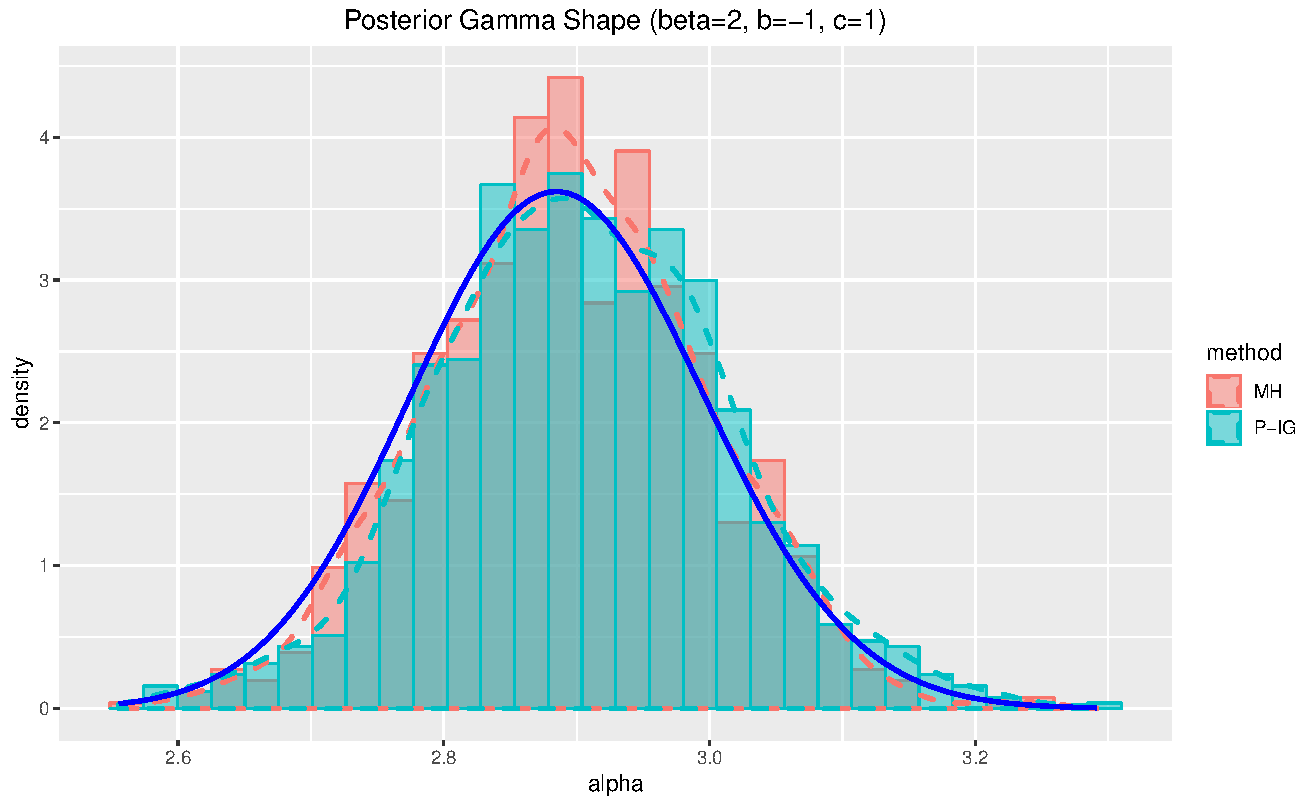
\includegraphics[width=0.75\linewidth,keepaspectratio=true]{gamma_shape_new.pdf}
\caption{Posterior of Gamma shape parameter. The green histogram shows posterior draws of our data augmentation model and the red ones shows that of a random-walk Metropolis Hastings sampler. Green/red dashed lines are empirical densities of posterior draws from two methods and blue solid line is the true posterior density.}
\end{center}
\label{fig:gammashape}
\end{figure}

\begin{figure}[htbp]
\centering
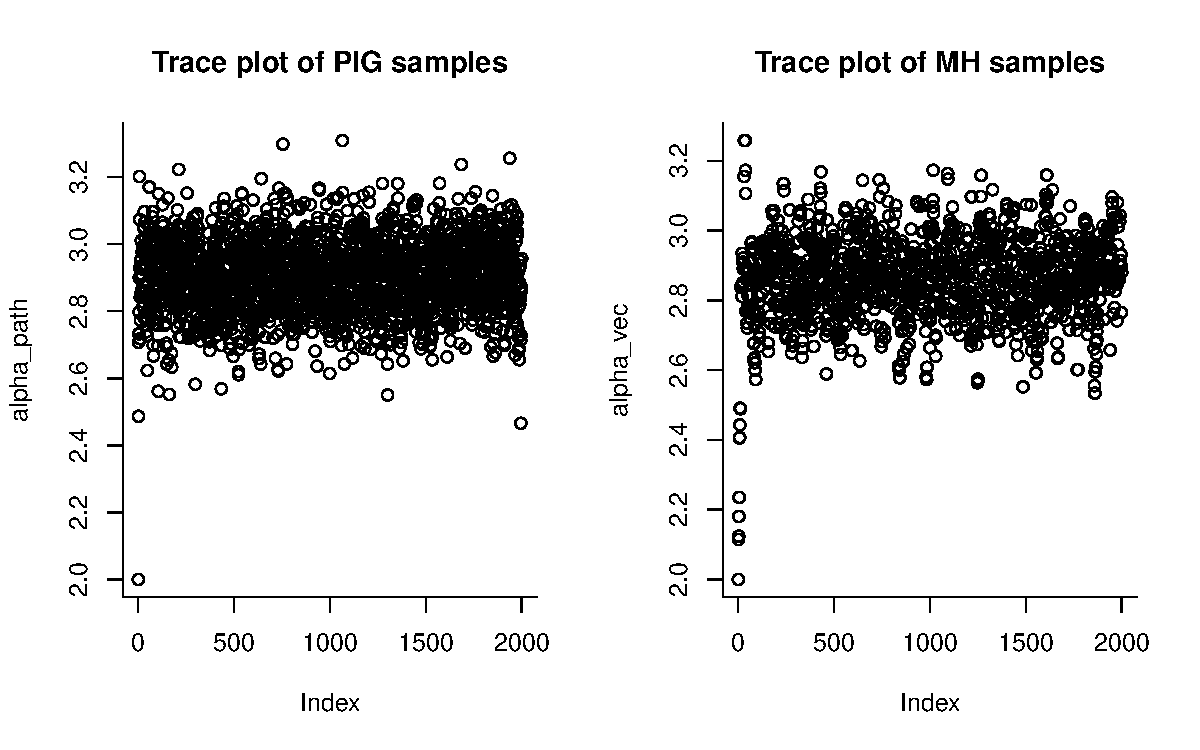
\includegraphics[width=0.8\textwidth]{gamma_shape_trace.pdf}
\caption{Trace plot of posterior draws from P-IG data augmentation sampler (left) and random-walk Metropolis Hastings sampler (right).}
\label{fig:gammashapetrace}
\end{figure}


\begin{figure}[htbp]
\centering
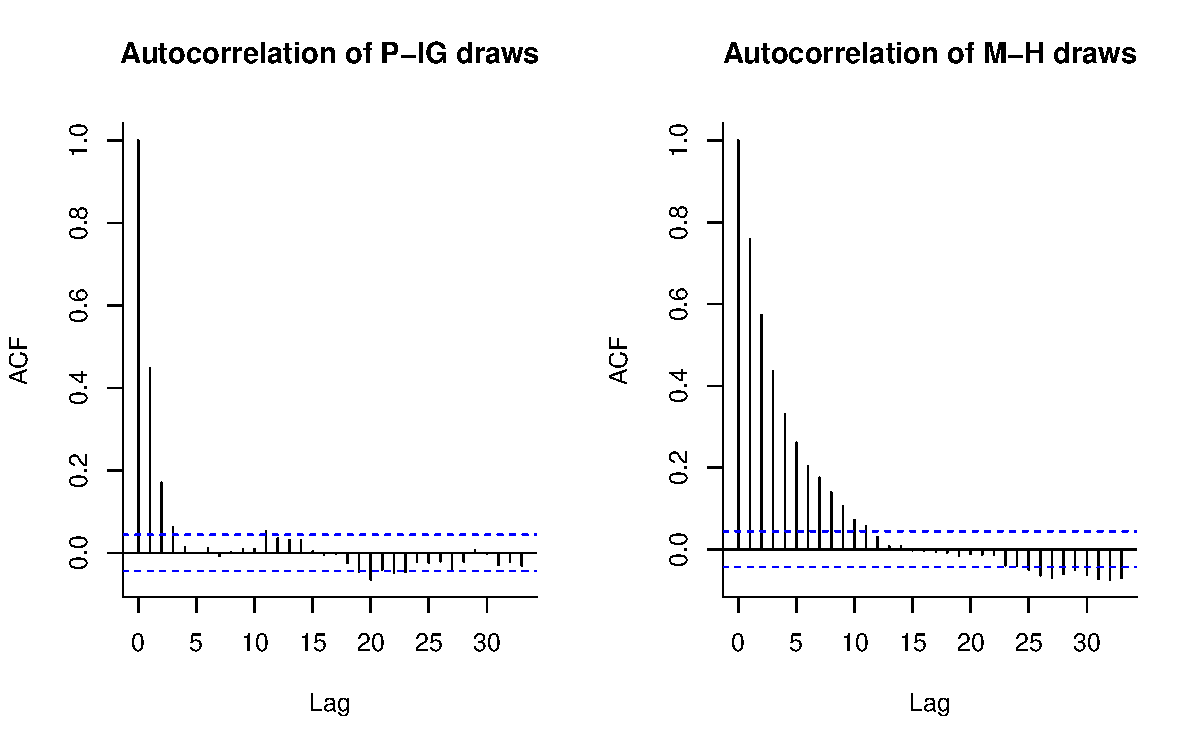
\includegraphics[width=0.8\textwidth]{gamma_shape_acf.pdf}
\caption{Autocorrelation of posterior draws from P-IG data augmentation sampler (left) and random-walk Metropolis Hastings sampler (right).}
\label{fig:gammashapeacf}
\end{figure}

Figure \ref{fig:gammashapetrace} and \ref{fig:gammashapeacf} show trace plot and autocorrelation of 2000 posterior samples by both samplers. While initializing at 2, the random-walk Metropolis-Hastings sampler can navigate to the posterior mode quickly because of the true density is single mode. However, the autocorrelation is large comparing to posterior draws of sampler with data augmentation. We also compute effective sample size by \texttt{R} package \texttt{coda}, the ratio of effective sample size to total posterior draws is 0.41 for our data augmentation strategy while it is only 0.14 for random-walk Metropolis Hastings algorithm.


\section{Application: Opioid and Prescription Drug Crisis}
\label{sec:Application}
We present an analysis of opioid and prescription drug abuse data to illustrate the applied utility of the data augmentation scheme devised in Section \ref{sec:Conentration_Inference}.  The opioid and prescription drug crisis continues to destroy lives in many parts of the United States. While the public discussion of the crisis focuses on opioid abuse, there are multiple drugs contributing to a larger pattern of substance abuse: cocaine, heroin, methadone, natural \& semi-synthetic opioids, psychostimulants, and synthetic opioids. Estimating shared patterns of variation in state-level mortality rates is particularly important to public health officials.  For example, identifying state-level characteristics associated with higher heroin overdose rates may inform public policy interventions.  To estimate the underlying pattern in mortality rates by drug type, we model death counts with the multinomial-Dirichlet framework presented in Section \ref{sec:Conentration_Inference}.  The data in our analysis comes from the \href{https://healthdata.gov/dataset/vsrr-provisional-drug-overdose-death-counts}{VSRR Provisional Drug Overdose Death Counts}, a nationwide data set on mortality statistics from 2015 - 2018. For 19 of 50 states, a break down of deaths by drug type is provided. The underlying overdose rates are not directly observed, and our inference goal is to learn shared patterns of variation in state-level death rates by drug type.  



\begin{table}
    \caption{\label{tab:VSRR}Deaths by drug type: cocaine, synthetic opioids, heroin, methadone, natural opioids, and psychostimulants. The data is provided at the state level from 2015 - 2018, and the snapshot provided above is the first six rows.}
  \centering
\fbox{%
\begin{tabular}{*{8}{c}}
\em State&\em Year&\em Cocaine&\em Synthetic&\em Heroin&\em Methadone&\em Nat.&\em Psych.\\
\hline
CT    & 2015 & 118     & 96        & 298    & 58        & 170  & 18     \\
CT    & 2016 & 171     & 240       & 403    & 72        & 180  & 24     \\
CT    & 2017 & 250     & 527       & 470    & 67        & 209  & 23     \\
CT    & 2018 & 280     & 682       & 405    & 97        & 180  & 39     \\
MD    & 2015 & 109     & 237       & 327    & 150       & 400  & 17     \\
MD    & 2016 & 154     & 386       & 418    & 179       & 394  & 21    \\ 
\end{tabular}}
\end{table}


Table \ref{tab:VSRR} provides a snapshot of the VSRR data, which reports a count vector for deaths across six different drug types at the state-year level.  Observe in Figure \ref{fig:overdose} that states/years exhibit distinct patterns of variation in empirical death proportion (ratio between the number of deaths by some drug and the total number of deaths).  In some states/years, the largest proportion of overdose deaths is from synthetic opioids, while in others it is heroin.  Significant state-year variation in normalized death counts motivates a hierarchical model for the proportion of deaths due to each drug type.     

\begin{figure}[h]
\centering
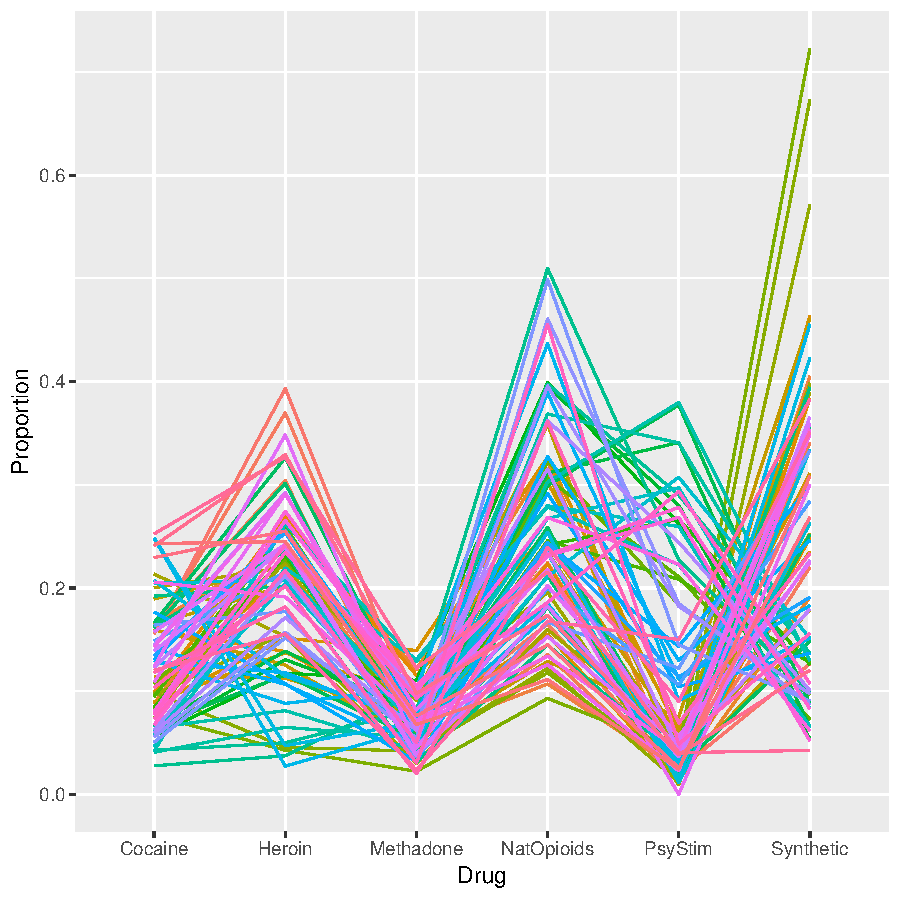
\includegraphics[width=6cm]{figure2.pdf}
\caption{Empirical proportion of overdose by drug type.}
\label{fig:overdose}
\end{figure}

In this analysis suppose that states and years are exchangeable, so that $m \in {1, \ldots, M}$ indexes each individual state-year combination.  Let $N_m$ denote the total number of overdose deaths in state-year $m$ due to the six drugs under consideration.  Let count vector $\nn_m$ denote the number of deaths associated with each drug type.  We model the count vector with a multinomial distribution conditional on the underlying state-year death proportions, 
\begin{align}
    \nn_m \mid \p_m \sim \text{Multinomial}\left(\p_m\right).
\end{align}

Probability vector $\p_m$ is the latent proportion of overdose deaths in each state-year associated with each drug type.  As observed in Figure \ref{fig:overdose}, variation in $\p_m$ at the state-year level is substantial, motivating a statistical model for $\p_m$ itself.  We elicit conditionally independent Dirichlet prior distributions for each $\p_m$, 
\begin{align}
    \p_m \mid \alphavec \sim \text{Dirichlet}\left(\alphavec\right).  
\end{align}
\begin{figure}[H]
\centering
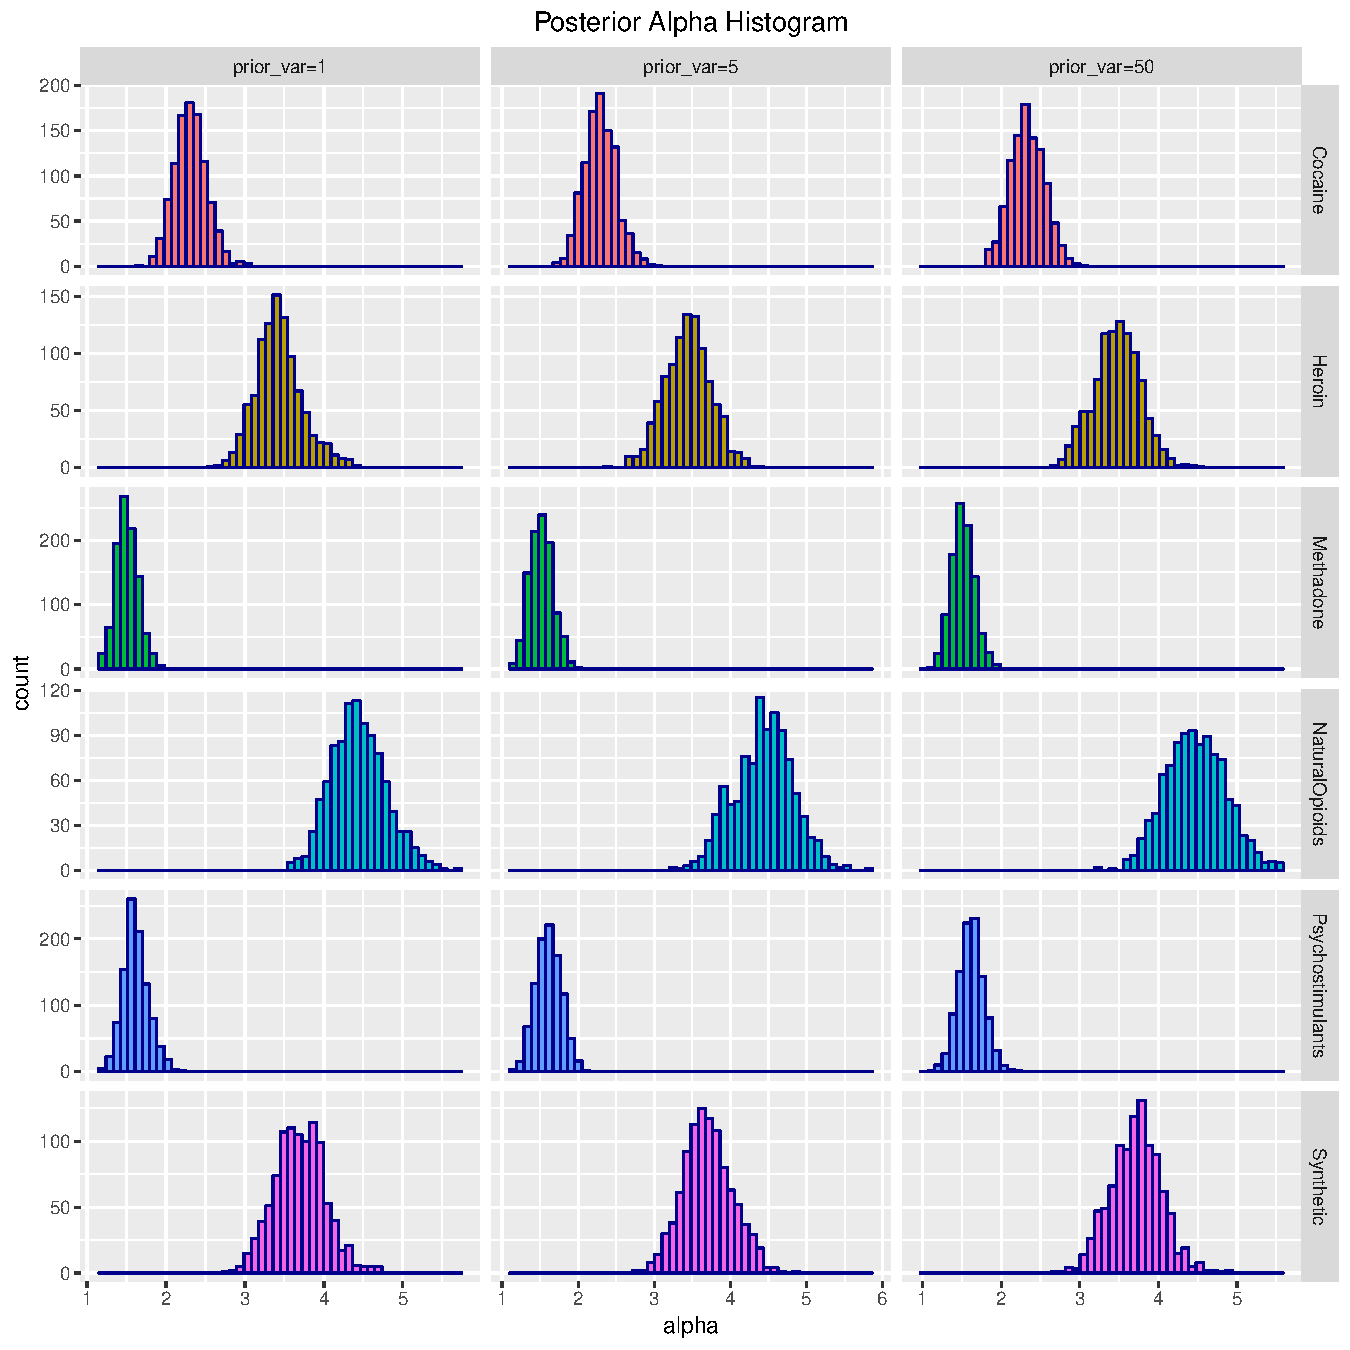
\includegraphics[width=0.6\textwidth]{opioid_var.pdf}
\caption{Posterior distributions for the concentration parameters $\alpha_k | \n_1, \ldots, \n_{76}$. Columns are posteriors under different choices of prior variance (prior expectation is fixed to be $1/K$).  The left column corresponds to the choice such that $Var[\alpha_k] = 1$; the middle column $Var[\alpha_k] = 5$; and the right column $Var[\alpha_k] = 50$.  Each row corresponds to the posterior $\alpha_k$ for one type of drug.}
\label{fig:opioid_var}
\end{figure}

\begin{figure}[H]
\centering
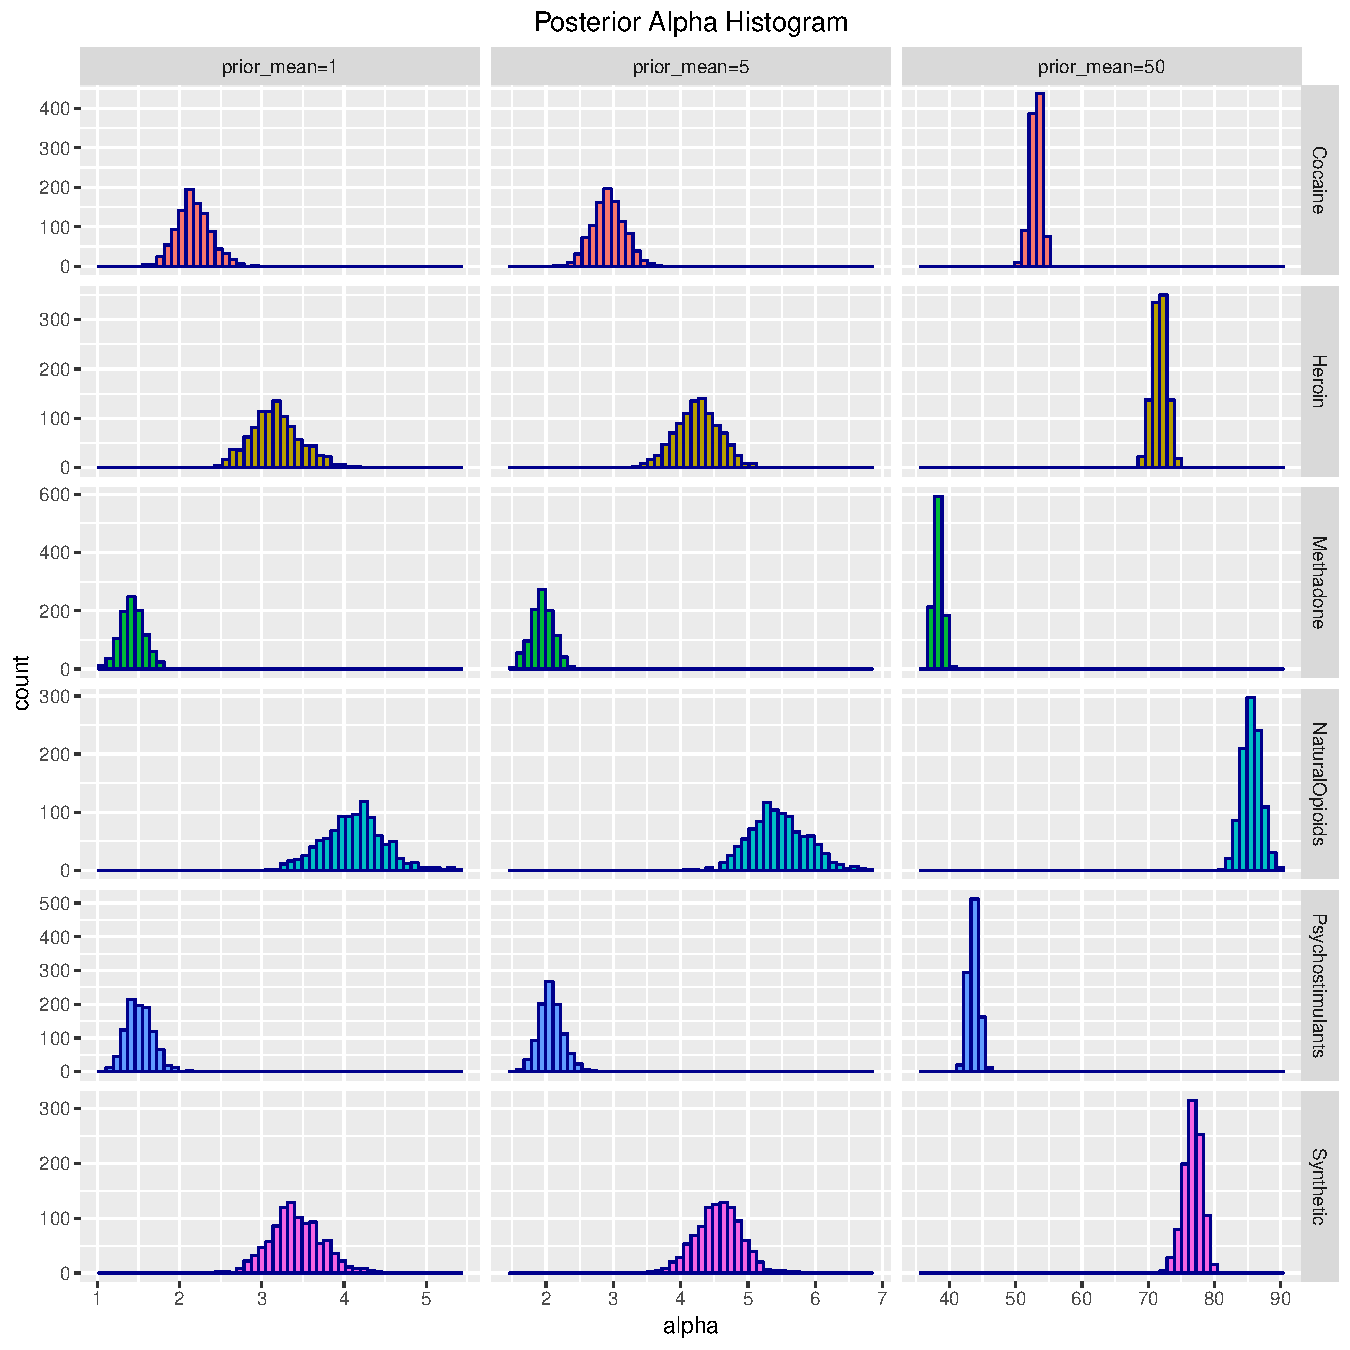
\includegraphics[width=0.6\textwidth]{opioid_mean.pdf}
\caption{Posterior distributions for the concentration parameters $\alpha_k | \n_1, \ldots, \n_{76}$. Columns are posteriors under different choices of prior expectation (prior variance is fixed to be $1$).}
\label{fig:opioid_mean}
\end{figure}

This hierarchical formulation enables the proportion of deaths associated with drug types to vary significantly from one state-year to the next.  The objective is to predict the proportion of deaths in a new state, $\p^*$, associated with each drug type.  The full posterior predictive distribution for $\p^*\mid \n_1, \ldots, \n_M$ quantifies (with uncertainty) the relative proportion of abuse-related deaths by drug type at the aggregate level. 

Following the algorithmic development in Theorem \ref{thm:theorem_2}, we first elicit gamma priors for $\alphavec$ with expectation $E[\alpha_k] = 1/K$ and different prior variances and compare the inferences (see Figure \ref{fig:opioid_var}).  Recall that when $\alpha_k \sim \Gamma(\tau, \beta)$, the prior expectation is $E[\alpha_k] = \tau / \beta$ and prior variance is $Var[\alpha_k] = \tau / \beta^2$. Observe in Figure \ref{fig:opioid_var} that as prior variance increases (with the smallest value in the left column), posterior estimates of $\alpha$ doesn't change much. Figure \ref{fig:opioid_mean} shows the alternative situations where the prior variance is  1 and the prior expectation varies. The posteriors now increases in magnitude, which reflects the increased prior variance, which reflects the increased prior expectation.  We also see in both Figure \ref{fig:opioid_var} and Figure \ref{fig:opioid_mean} that the posterior distributions for the concentration parameters associated with heroin, natural opiods, and synthetic opiods are relatively larger than the concentration parameters for cocaine, methadone, and psychostimulants.  In Figure \ref{fig:opioid_mean}, as the expected value of the concentration parameter increases from 1 in the left column of to $50$ in the right column, the separation of the posteriors becomes more pronounced.  

\begin{figure}[H]
\centering
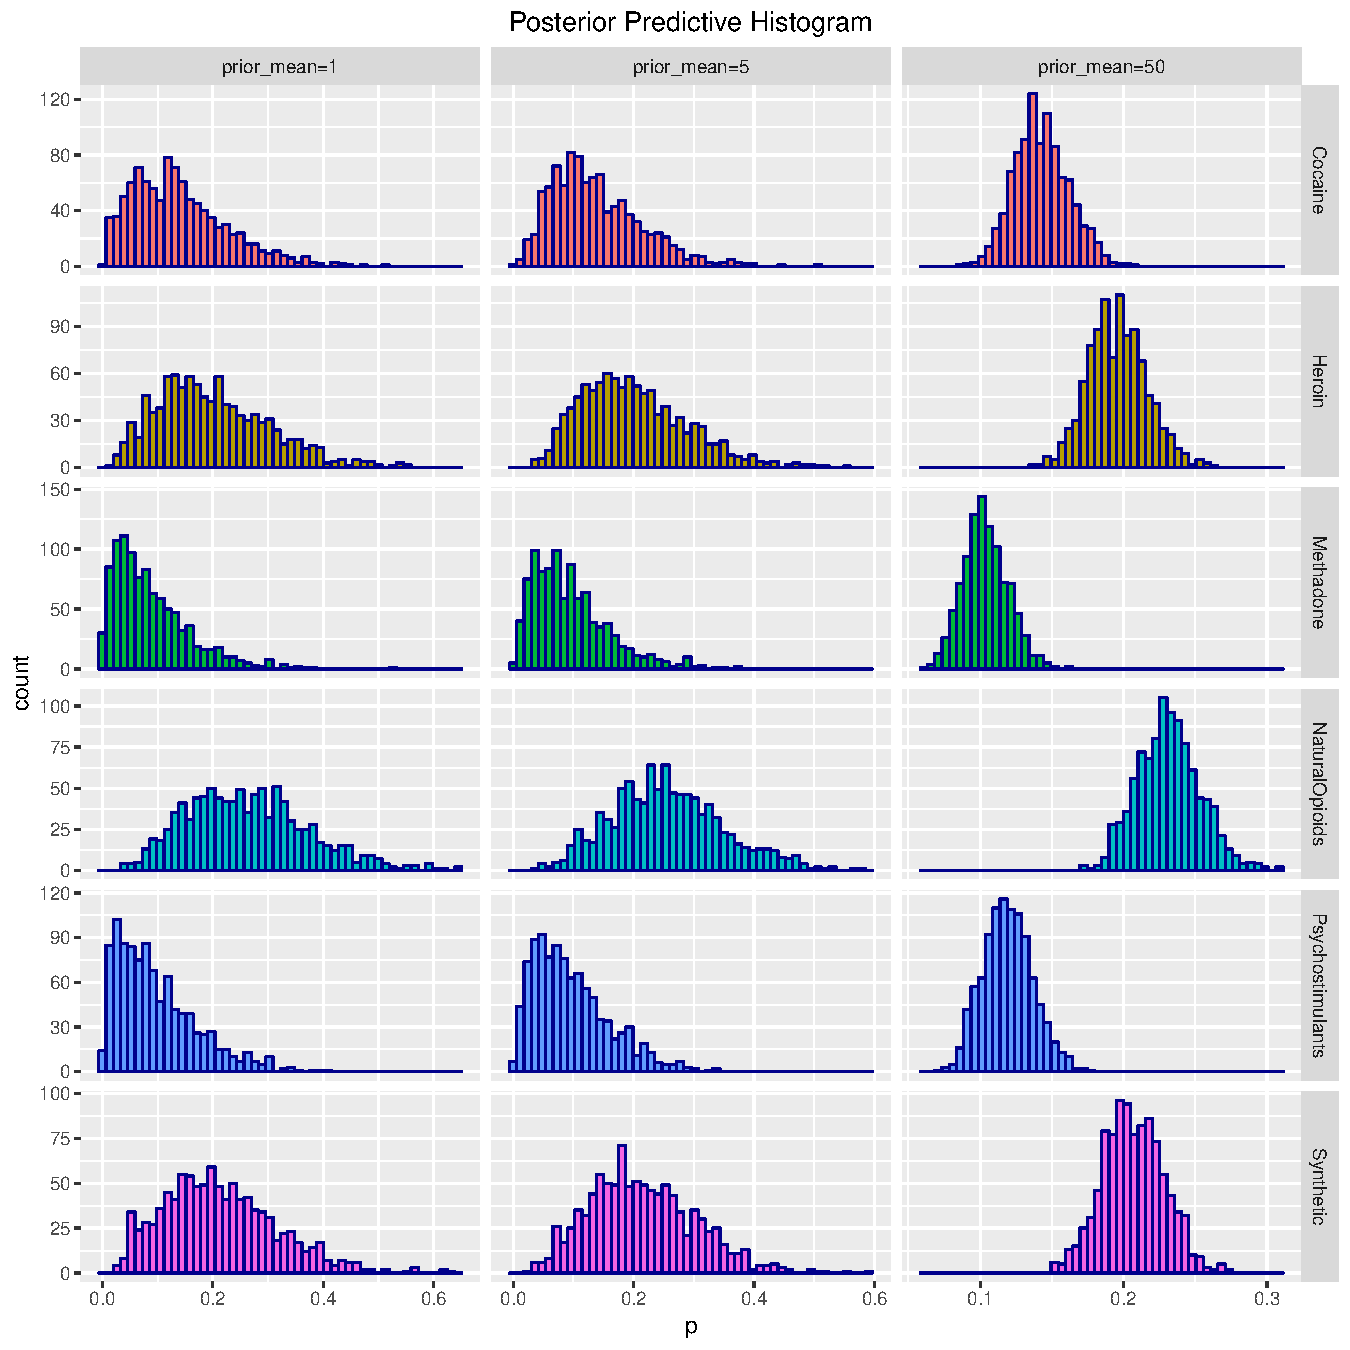
\includegraphics[width=0.6\textwidth]{opioid_predictive_new.pdf}
\caption{Posterior predictive distribution of $\p$, with gamma on $\alpha$. Prior variance is $1$. Prior expectation is $1, 10$ and $50$, same as Figure \ref{fig:opioid_mean}.}
\label{fig:opioid_predictive}
\end{figure}

Computing the posterior for each $\alpha_k$ facilitates computation of a posterior predictive distribution for the proportion of deaths in a new state-year associated with each drug type.  Rather than fixing $\alpha_k$, we estimate the $\alpha_k$ and propagate uncertainty in the concentration parameters to predictions about the proportion of deaths attributed to each drug.  Figure \ref{fig:opioid_predictive} illustrates that the posterior predicted proportion of deaths associated with heroin, natural opioids, and synthetic opioids is again relatively larger than the predictive values for cocaine, methadone, and psychostimulants, under the setting of fixed prior variance and varying prior expectation. Since the priors for $\alpha_k$'s are i.i.d.,  the prior specification of all  three columns concentrate the predictive mass around uniform $\p$, i.e. $p_k = 1/K\approx 0.167$ for $k=1,2,...,6$. The larger value of prior expectation of $\alpha_k$ means that the prior distribution of $p_k$ is more concentrated. This is clearly illustrated in the right hand column of Figure \ref{fig:opioid_predictive}, whose prior mean of each concentration parameter has the largest magnitude, $E[\alpha_k] = 50$, and accordingly the posterior predictive distributions of $p_k$'s have the smallest spread among the three columns.

\section{Discussion}
\label{sec:Discussion}
The P\'olya-inverse Gamma distribution facilitates fully Bayesian posterior inference for concentration and shape parameters in Dirichlet and gamma statistical models, respectively.  The P-IG distribution class is flexible and admits fast and efficient stochastic simulation methods in widely-used statistical models, such as latent Dirichlet allocation, Gamma-Gamma hierarchical models, and Bayesian nonparametric mixture models.  The P-IG$\left(c\right)$ distribution is constructed from an infinite convolution of GIG distributions. Our parameter expanded Gibbs sampler leverages the scale mixture of normals representation of the P-IG distribution to estimate parameters nested in the gamma function.      

The focus of the current paper is on theoretical and algorithmic development of the P-IG distribution class.  Our work builds on distributional results of \citet{hartman1976completely} and \citet{roynette2005couples} and contributes to the literature on scale mixtures of normals (see, e.g., \cite{andrews1974scale, west1987scale, polson2013bayesian}).  We believe that the computational strategies developed here will provide the foundation for new and richly structured hierarchical models of Dirichlet concentration and gamma shape parameters.  Applied Bayesian analyses of categorical data will benefit from increased model flexibility and information borrowing strategies.       

There are a number of avenues for future research. In particular, regularized scale allocation models can be implemented using data augmentation methods of \cite{polson2013data} with P-IG distribution. \cite{barndorff1992multivariate} provide multivariate GIG distribution theory and relationships with Poisson processes.

\bibliographystyle{rss}
\bibliography{PGgamma} 


\newpage
\appendix
\section{Proof of Lemma \ref{lemma1}}\label{lemma_proof}
Let $W_k \sim IG(\frac{3}{2}, \frac{1}{2k^2})$. It has density 
$$
f_{W_k}(y) = \frac{1}{\Gamma(\frac{3}{2})(4k^2)^{\frac{3}{2}}}  y^{-\frac{5}{2}} e^{-\frac{1}{4k^2} y^{-1}}, 
$$
so that with $t\geq 0$,
\begin{equation*}
\begin{aligned}
E(e^{-t^2 W_k}) &= \int_0^\infty e^{-t^2 y}  \frac{1}{\Gamma(\frac{3}{2})(4k^2)^{\frac{3}{2}}}  y^{-\frac{5}{2}} e^{-\frac{1}{4k^2} y^{-1}} dy\\
&=  \left( 1 + \frac{t}{k} \right) e^{-\frac{t}{k}}.
\end{aligned}
\end{equation*}
Therefore, by construction,
\begin{equation*}
W \overset{d}{=} \sum_{k=1}^\infty W_k
 \Longleftrightarrow E(e^{-t^2 w}) = \prod_{k=1}^\infty \left( 1 + \frac{t}{k} \right) e^{-\frac{t}{k}}.
\end{equation*}
by the uniqueness of Laplace transform.


\section{Proof of Theorem \ref{thm:theorem_1}}\label{proof_thm1}
It suffices to show that if $X_k\sim GIG\left(-\frac{3}{2}, 2c^2, \frac{1}{2k^2}\right)$, then the following integral identity holds, 
$$
E(e^{-t^2 X_k}) = \left( \frac{k + \sqrt{t^2 + c^2}}{k + c} \right) e^{-\frac{\sqrt{t^2 + c^2}-c}{k}}.
$$
The density of $X_k$ given by
$$
f_{k, c}(x) = m\left(k, c\right) x^{-\frac{5}{2}} \exp\left(-\frac{1}{4k^2x}  - c^2x\right).
$$ with normalizing constant, $$m(k, c) = \frac{1}{\Gamma\left(\frac{3}{2}\right)}\frac{ (2k)^{-3}}{c k^{-1} +1}e^{c k^{-1}}.$$ 
It follows by the algebraic calculation,
\begin{align*}
\int_0^\infty e^{-t^2 x} f_{k, c}(x) dx &= m(k, c) \int_0^\infty  x^{-\frac{5}{2}} \exp\left(-\frac{1}{4k^2} x^{-1} -(t^2 + c^2) x\right) dy \\
&= \frac{m(k, c)}{m\left(k, \sqrt{t^2 + c^2}\right)}\\
&= \frac{(\sqrt{t^2 + c^2} k^{-1} +1) \exp\left(\sqrt{t^2 + c^2} k^{-1}\right)}{(c k^{-1} +1)\exp( ck^{-1})}\\
&=  \left( \frac{k + \sqrt{t^2 + c^2}}{k + c} \right) e^{-\frac{\sqrt{t^2 + c^2}-c}{k}},
\end{align*}
as required.

\section{Proof of Theorem \ref{thm:theorem_2}} \label{proof_thm2}
Let there be $K$ classes and $M\times K$ count observations,  where $n_{mk}$ is the count of $k$-th class in the $m$-th instance and $p_{mk}$ the underlying probability. $\alpha = (\alpha_1, \alpha_2, ..., \alpha_K), \alpha_0 = \sum_{k=1}^K \alpha_k$. The model is as follows, for $m=1, 2, ..., M$,
\begin{align*}
\p_m | \alphavec & \sim \text{Dirichlet}(\alpha_1, \alpha_2, ..., \alpha_K)\\
\n_m | \p_m & \sim \text{Multinomial}(p_{m1}, p_{m2}, ..., p_{mK})
\end{align*}
where $\n_m = (n_{m1}, n_{m2}, ..., n_{mK})', \p_m = (p_{m1}, p_{m2}, ..., p_{mK})'$. 
We assume $\p_m$ are independent across $m$ given $\alphavec$, and $\n_m$ independent across $m$ given $\p$. Also, given $\p_m$, $\n_m$ is independent of $\alphavec$. Now we consider the posterior density $f(\alphavec|\n)$, with $\n = (\n_1, \n_2, ..., \n_M)$.
\begin{align*}
f(\alphavec | \n) &= \int f(\alphavec, \p | \n) d\p\\
&= \int \frac{f(\alphavec)f(\p|\alphavec)f(\n|\p)}{f(\n)} d\p \\
&= \frac{f(\alphavec)}{f(\n)} \int \prod_{m=1}^M f(\p_m|\alphavec)f(\n_m|\p_m) d\p\\
&= \frac{f(\alphavec)}{f(\n)C(\n)} \int \prod_{m=1}^M \left(\frac{\Gamma(\alpha_0)}{\prod_{k=1}^K \Gamma(\alpha_k)}\prod_{k=1}^K p_{mk}^{\alpha_k-1} \right)\left(\prod_{k=1}^K p_{mk}^{n_{mk}}\right)   d\p\\
&= \frac{f(\alphavec)}{f(\n)C(\n)} \int \prod_{m=1}^M \left(\frac{\Gamma(\alpha_0)}{\prod_{k=1}^K \Gamma(\alpha_k)}\prod_{k=1}^K p_{mk}^{\alpha_k+n_{mk}-1} \right) d\p\\
&= \frac{f(\alphavec)}{f(\n)C(\n)} \int \prod_{m=1}^M \left(\int_0^\infty \eta_m^{\alpha_0 - 1} e^{-\eta_m} d \eta_m \prod_{k=1}^K \int_0^\infty \alpha_k e^{\gamma\alpha_k} e^{-\alpha_k^2 w_{mk}}f(w_{mk})dw_{mk}\prod_{k=1}^K p_{mk}^{\alpha_k+n_{mk}-1} \right) d\p\\
&=  \int f(\alphavec, \p, \eeta, \w | \n)d\p d\eeta d\w\\
\end{align*}
where $C(\n) = \prod_{m=1}^M \frac{\prod_{k=1}^K \Gamma(n_{mk}+1)}{\Gamma(1 + \sum_{k=1}^M n_{mk})}$,
\begin{align*}
f(\alphavec, \p, \eeta, \w | \n) &\propto \left(f(\alpha) \prod_{k=1}^K \alpha_k^M e^{M\gamma\alpha_k} \right)\prod_{m=1}^M  \left( \eta_m^{\alpha_0 - 1} e^{-\eta_m}  \prod_{k=1}^K   e^{-\alpha_k^2 w_{mk}}f(w_{mk})\prod_{k=1}^K p_{mk}^{\alpha_k+n_{mk}-1} \right), 
\end{align*}
and $f(w_{mk})$ is the density of P-IG(0). 
Now we assume independent gamma priors, $f(\alphavec) \propto \prod_{k=1}^K \alpha_k^{\tau-1}e^{-\beta \alpha_k}$. Then simply re-organizing the above expression of $f(\alphavec, \p, \eeta, \w | \n)$ gives

\begin{align*}
f(\alpha_k | \p, \w, \eeta, \n) &\propto  \alpha_k^{\tau + M - 1} \exp\left\{-\left(\sum_{m=1}^Mw_{mk}\right)\alpha_k^2 + \left(M\gamma - \beta + \sum_{m=1}^M \log(\eta_m p_{mk})\right)\alpha_k\right\},\\
f(\p_{m} | \alphavec, \w, \eta, \n) &\propto \prod_{k=1}^K p_{mk}^{\alpha_k+n_{mk}-1},\\
f(\eta_m | \alphavec, \p, \w, \n)  &\propto \eta_m^{\alpha_0 - 1} e^{-\eta_m}, \\
f(w_{mk} | \alphavec, \p, \eeta, \n) &\propto e^{-\alpha_k^2 w_{mk}}f(w_{mk}).
\end{align*} 

\section{Sampling from Conditional Posterior of $\alpha$} \label{sample_alpha}
The probability density of a random variable $H(m, a, b)$ is given as 
$$
h(x|m,a,b) = \frac{x^{m-1}e^{-ax^2+bx}}{\int_0^\infty x^{m-1}e^{-ax^2+bx}dx},\; (x, m,a >0, b\neq 0).
$$
Note that we can write it as a multiplication 
\begin{align*}
h(x|m,a,b) &=   \frac{x^{m-1}e^{-ax^2+bx}}{\int_0^\infty x^{m-1}e^{-ax^2+bx}dx} \\
&=  \frac{x^{m-1}e^{-(\tau|b|-b)x}e^{-a(x - \tau|b|/2a)^2}}{\int_0^\infty x^{p-1}e^{-(\tau|b|-b)x}e^{-a(x - \tau|b|/2a)^2}dx}\\
& = ce^{-a(x - \tau|b|/2a)^2}g(x|p,\tau|b|-b) 
\end{align*}
where $g(x|m,b)$  is the density of a gamma random variable with shape $m$ and rate $\tau|b|-b > 0$. $$0\leq e^{-a(x - \tau|b|/2a)^2} \leq 1,\, c =\frac{\int_0^\infty x^{p-1}e^{-(\tau|b|-b)x}dx}{\int_0^\infty x^{p-1}e^{-(\tau|b|-b)x}e^{-a(x - \tau|b|/2a)^2}dx} \geq 1$$
We sample from $h(x)$ by rejection method: 
\begin{enumerate}
\item Generate $X\sim \Gamma(m, \tau|b|-b)$ and $U\sim Unif[0,1]$
\item Return $X$ until $U \leq e^{-a(X - \tau|b|/2a)^2}$.
\end{enumerate}
If $b>0$, we set $\tau = \sqrt{1/4 + 2am/b^2} + 1/2$; if $b<0$, we set $\tau = \sqrt{1/4 + 2am/b^2} - 1/2$. Then $e^{-a(E(X) - \tau|b|/2a)^2} = 1$.

\end{document}